\section{Pre-lab tasks}
% Q5.1
Using equation \eqref{math:Gammaf}, one finds
\begin{equation}
	\Gamma_e = \Gamma_\mu = \Gamma_\tau = \SI{83.40}{\mega\eV}
\end{equation}
The decay widths to leptons of three generations are the same because of lepton universality and neglecting the masses. With the same equation, decay width to quarks in total is
\begin{alignat*}{2}
	\Gamma_u &= \Gamma_c &&= \SI{285.34}{\mega\eV} \\
	\Gamma_d &= \Gamma_s = \Gamma_b &&= \SI{367.79}{\mega\eV}
\end{alignat*}
It is significantly larger, since there are more quarks in SM and quarks carry more degrees of freedom (color) than leptons. Decays to neutrinos are invisible for detector in LEP, but still they have the width of
\begin{equation}
	\Gamma_{\nu} = \SI{165.84}{\mega\eV}
\end{equation}

% Q5.2
Hadronic part
\begin{equation}
	\Gamma_\text{h} = \sum_{\forall q\neq t} \Gamma_q = \SI{1674.06}{\mega\eV}
\end{equation}
Charged decay
\begin{equation}
	\Gamma_\text{charged} = 3 \Gamma_e = \SI{250.17}{\mega\eV}
\end{equation}
Invisible decay
\begin{equation}
	\Gamma_\text{inv} = 3\Gamma_\nu = \SI{497.52}{\mega\eV}
\end{equation}
In total (except unknown decays)
\begin{equation}
	\Gamma_\text{total} = 3\Gamma_e + \Gamma_h + 3\Gamma_\nu = \SI{2421.75}{\mega\eV}
\end{equation}

\begin{table}[ht]
	\centering
	\label{tab:label}
	\begin{tabular}{ccc}
		\toprule
		decay type & partial width/\si{\mega\eV} & partial cross section/$10^{-5}\si{\mega\eV\tothe{-2}}$	 \\
		\midrule
		hadronic & \num{1674.06} & \num{10.79} \\
		charged & \num{250.17} & \num{1.61} \\
		invisible & \num{497.52} & \num{3.21}  \\
		total & \num{2421.75} & \num{15.61} \\
		\bottomrule
	\end{tabular}
	\caption{Decays widths and partial cross sections}
\end{table}


% Q5.3
Assume that there is another generation of light fermions, the total width of $Z^0$ would be
\begin{equation}
	\Gamma'_\text{total} = \Gamma_\text{total} + \Gamma_e + \Gamma_\nu + \Gamma_u + \Gamma_d = \SI{3324.11}{\mega\eV}
\end{equation}
It would be a change of $37 \%$ percent!

% Q5.4
The differential cross section $\dv{\sigma}{\Omega}$ has different angular dependencies for $s$- and $t$-channels, see equations \eqref{math:diffCrossS} and \eqref{math:diffCrossT}. Simply plotting without the proportional constant in front shows where $s$- or $t$-channels dominates the process, see figure.~\ref{fig:angDep}.
\begin{figure}[ht]
	\centering
	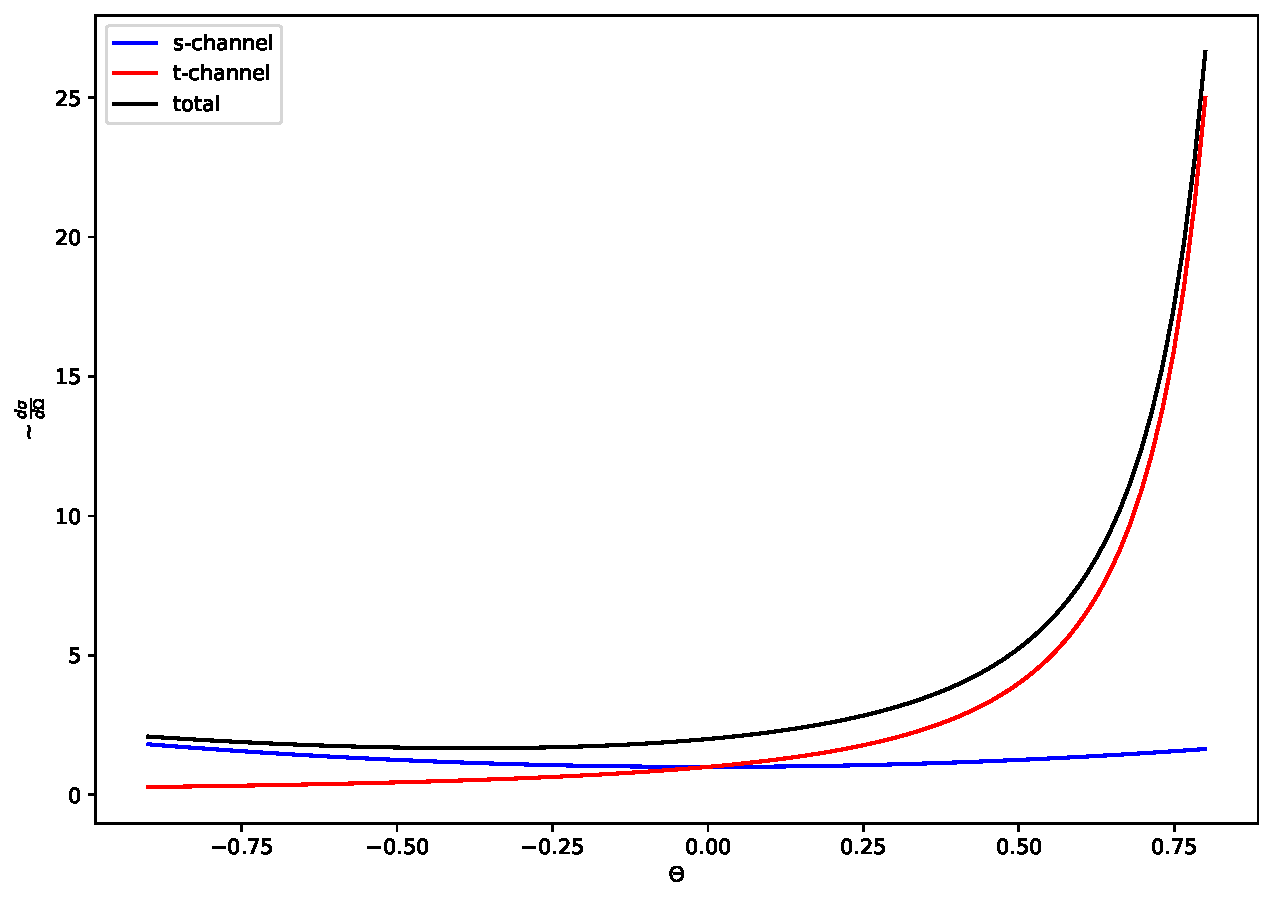
\includegraphics[width=0.8\linewidth]{angDep.pdf}
	\caption{Angular dependencies of two channels.}%
	\label{fig:angDep}
\end{figure}
At small angles, $t$-channel dominates, whereas at large angles, $s$-channel dominates.
